\begin{section}{Power Spectra and Information Content}
  \label{sec:fisherinfo}
    The power spectrum is the Fourier transform of the correlation function and measures
 the amount of clustering in the matter distribution as a function of wavenumber $k$,
\begin{align}
    \langle \delta \left( \bm{k} \right) \delta \left( \bm{k'}\right) \rangle =
\left( 2\pi \right) ^3 P \left( \bm{k} \right) \hat{\delta} \left( \bm{k}-\bm{k'} \right),
\end{align}
where $\delta \left( \bm{k} \right)$ is the density fluctuation in wave space, while 
$\hat{\delta}$ is the delta funciton. Of equal interest is $\Delta ^2(k)$, the power 
spectrum in its dimensionless form, defined as
\begin{align}
    \Delta ^2(k) \equiv \frac{k^3 P \left( k \right)}{2\pi ^2}.
\end{align}
    The power spectra of the mass distributions are calculated using the \enquote{\textit{Nearest Grid Point}} 
(NGP) mass assignment scheme. In Fig.\ref{fig:cross-correlation-power}(a) we plot the mean cross correlation 
function, $r=P_{\delta \delta_L}/\sqrt{P_\delta P_{\delta_L}}$ of the nonlinear and the 
linear power spectrum, and the reconstructed and 
linear power spectrum respectively. The wave number where the cross correlation drops to a half increases 
from $k\simeq$ 0.2 $h/\mathrm{Mpc}$ to $k \simeq$ 0.6 $h/\mathrm{Mpc}$. 
To qualify the improvement of cross correlation in the 
power spectrum, we compute the damping factors $\mathcal{D}(k)=r^4$ fitting the Gaussian BAO damping models 
$\mathcal{D}(k)=\mathrm{exp}(-k^2 \Sigma^2/2)$. In Fig.\ref{fig:cross-correlation-power}(a) 
we plot $\mathcal{D}_\delta^{1/4}$ ($\Sigma =$ 11.3 $\mathrm{Mpc}/h$) and $\mathcal{D}_{\delta_R}^{1/4}$ 
($\Sigma = $ 3.9 $\mathrm{Mpc}/h$) over $r_{\delta\delta_L}$ and $r_{\delta_R\delta_L}$. 
We also plot $\mathcal{D}(k)^{1/4}$ 
that match cross correlation function after $E$-mode displacement 
reconstruction result in \cite{bib:Yu2016} ($\mathrm{ng}=512$, box size $=$ 400 $\mathrm{Mpc}/h$, $\Sigma =$ 1.3 $\mathrm{Mpc}/h$), and 
MM reconstruction result in a higer resolution in \cite{bib:ZhuH2016} ($\mathrm{ng}=512$, 
box size $=$ 600 $\mathrm{Mpc}/h$, $\Sigma =$ 2.6 $\mathrm{Mpc}/h$), 
which is the result in \cite{bib:ZhuH2016}. We find that in higher resolution, 
the reconstruction gives a cross correlation damping at smaller scale. 
And it's expected that the $E$-mode displacement reconstruction gives a reconstructed power spectrum more correlated 
with the initial one, since it completely picks out the irrotational components of the real displacement 
field in $N$-body simulation, while through MM reconstruction, the difference between the reconstructed displacement 
and the real displacement still contains an irrotational component, which is also correlated with the linear power spectrum.
 In Fig.\ref{fig:cross-correlation-power}(b) we plot the linear power spectrum which is the transfer function, and mean 
power spectrum (with error bars) of 136 nonlinear density fields and reconstruced density fields simply 
given by $\delta_R=\Delta^2\phi$. The reconstructed power spectrum drops at nonlinear scale ($k \gtrsim$ 0.3 $h/\mathrm{Mpc}$) 
since the reconstructed density fields are totally irrotational. The result is similar to that of 
$E$-mode displacement reconstruction described in \cite{bib:Yu2016}, in which the reconstructed power spectrum 
drops, but in a different scale and at a different speed.
\begin{figure*}
%\begin{subfigure}[b]{0.48\textwidth}
\centering
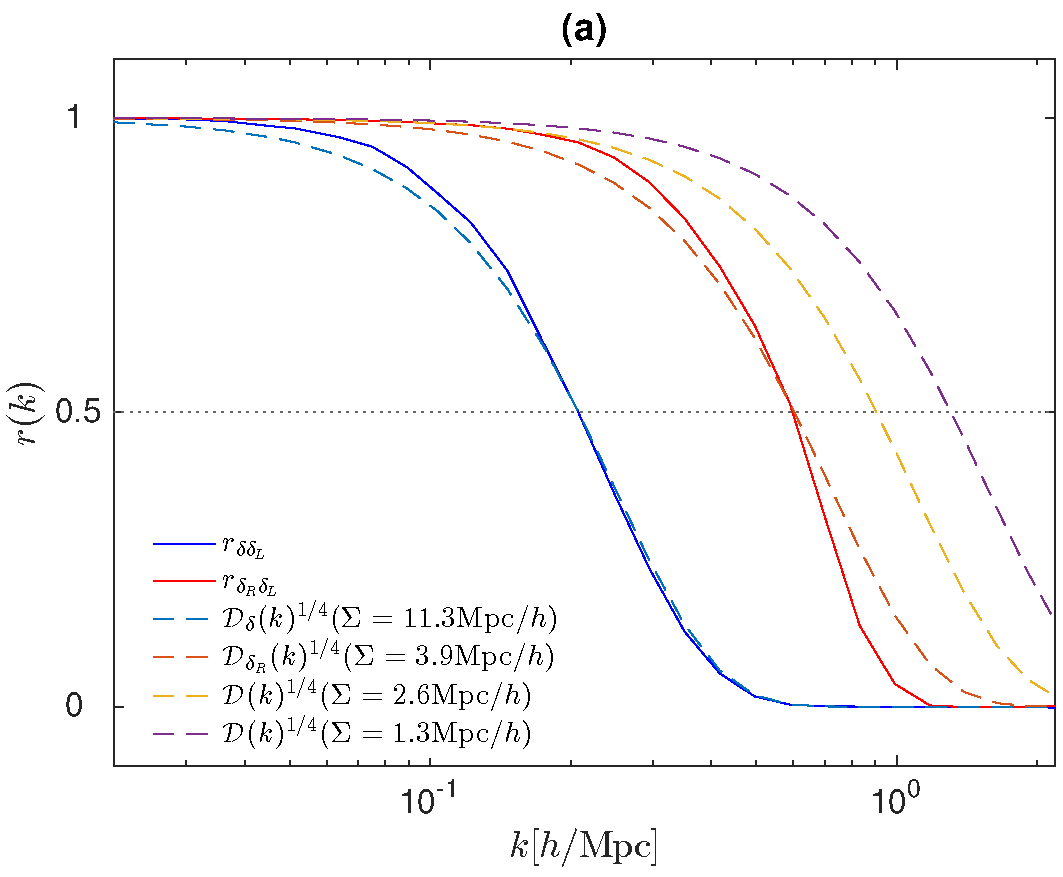
\includegraphics[width=0.455\textwidth]{cross_correlation_best_analysis-crop.pdf} 
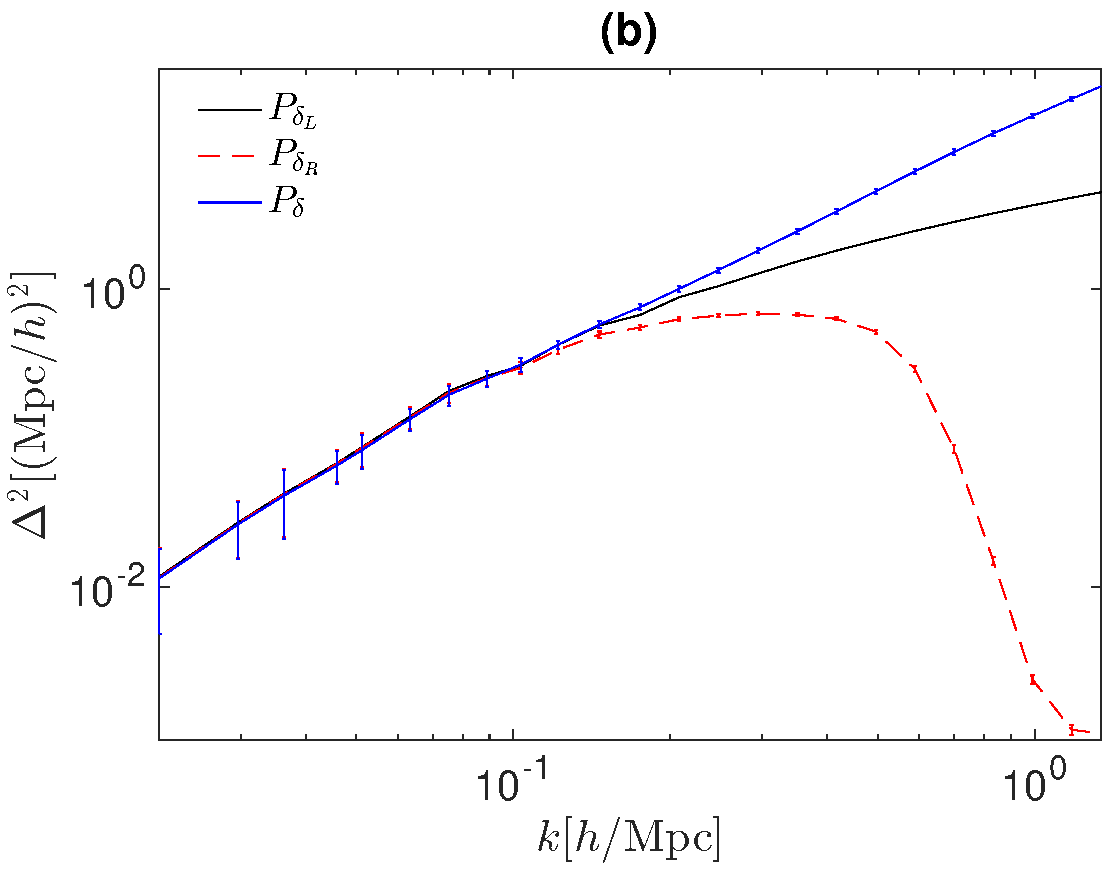
\includegraphics[width=0.48\textwidth]{power_best_analysis-crop.pdf}
%\includegraphics[width=0.5\textwidth]{power_nberror-crop.pdf}
\caption{(a) The cross correlation function (solid lines) $r_{\delta\delta_L}$ (blue) and $r_{\delta_R\delta_L}$ (red), 
and BAO damping models (dash lines). 
(b) The dimensionless power spectrum computed via linear theory (black), the mean value of 136 $N$-body simulations
with $1\sigma$ error bars (blue), and reconstruction of the simulations (red).}
\label{fig:cross-correlation-power}
\end{figure*}

   Mathamatically, the Fisher information \cite{bib:Tegmark1997} $I$ in the log of amplitude $A$ of the initial 
matter power spectrum is defined as 
\begin{align}
   I_A \equiv -\left\langle \frac{\partial ^2 \mathrm{ln \Largr}}{\partial A ^2}\right\rangle,
\label{eq:fisherdefine}
\end{align}
   in which $\Largr$ denotes the likelihood. For Gaussian fluctuations, the likelihood depends on
parameters only through the power spectrum $P(k)$, and the information $I$ in A defined by Eq.\ref{eq:fisherdefine}
can be written as \cite{bib:Rimes2006}
\begin{align}
    I_A = - \left\langle \sum_{k,k'} \frac{\partial \mathrm{ln} P(k)}{\partial \mathrm{ln} A} 
\frac{\partial ^2 \mathrm{ln \Largr}}{\partial \mathrm{ln} P(k) \partial \mathrm{ln} P(k')}
\frac{\partial \mathrm{ln} P(k')}{\partial \mathrm{ln} A}\right\rangle,
\label{eq:fisherdefineforgaussian}
\end{align}
in which the angle bracket denotes the average over all the power spectra.

  The definition Eq.\ref{eq:fisherdefineforgaussian} can be written in a simpler form in two aspects, one 
of which is the first and the third partial dericative terms. 
For any density field $\delta$, we can conveniently decompose it into linear and nonlinear components
\begin{align}
    \delta (k) = b (k) \delta _L (k) + n (k),
\label{eq:decompose}
\end{align}
in which $\delta_L$ denotes the linear density field. $b (k)$ is the bias and $n (k)$ is defined  
such that the correlation $\langle \delta_L (k) n (k) \rangle$ is zero. If we correlate  
$\delta$ and $\delta_L$,
\begin{align}
   \langle \delta (k) \delta_L (k) \rangle = b (k) \langle \delta_L (k) \delta_L (k) \rangle,
\label{eq:correlating}
\end{align} 
    we can solve for $b$ as 
\begin{align}
    b (k) = \frac{P _{\delta \delta_L}(k)}{P_{\delta_L}(k)}.
\label{eq:bofk}
\end{align}
Non-linear evolution drives $b (k)$ to drop from unity, and generates the nonlinear term $n (k)$. 
Correlating $\delta$ and itself, 
\begin{align}
  \langle \delta (k) \delta (k) \rangle = b^2 (k) \langle \delta_L (k) \delta_L (k) \rangle + \langle n(k)n(k) \rangle,
\end{align}
we find 
\begin{align}
   P_\delta (k) = \mathcal{D} (k) P_{\delta_L} (k) + P_n (k),
\label{eq:powerdecompose}
\end{align}
where $\mathcal{D}(k) \equiv b^2 (k)$ is the nonlinear damping factor, and $P_n$ is the mode coupling term.

   With the help of Eq.\ref{eq:bofk} and Eq.\ref{eq:powerdecompose}, we can replace the partial derivatives 
$\partial \mathrm{ln} p(k) / \partial \mathrm{ln} A$ in Eq.\ref{eq:fisherdefineforgaussian} with 
\begin{align}
   \frac{A}{P(k)}\frac{\partial P(k)}{\partial A}=\frac{P_{\delta \delta_L}^2(k)}{P_\delta(k) P_{\delta_L}(k)}
\end{align}
which is just the square of the 
cross correlation function $r ^2 (k)$, of $\delta$ and $\delta_L$. 

The second partial derivative terms in 
Eq.\ref{eq:fisherdefineforgaussian}, the Hessian of the vector $\mathrm{ln} P(k)$, has the expectation 
value of the Fisher matrix with respect to the log powers. For linear density fields, the Fisher matrix is 
approximately equal to the inverse of the covariance matrix of power spectrum estimates, which should be diagonal, 
with diagonal elements equal to the number of modes in each wavenumber bin (when considering $\bm{k}$ and $-\bm{k}$ 
as the same mode). Thus we can write down a simpler matrix product form of cumulative Fisher information, 
\begin{align}
    I_A \left( < k_n\right) = r^2(k)^{\mathrm{T}} \left[ \mathrm{C^{-1}_{norm}} ( k,k' )\right] r^2(k') ,
\label{eq:fisherformulaused}
\end{align}
where $\mathrm{C_{norm}}$ is the normalized covariance matrix with size per dimension up to $k_n$, defined as
\begin{align}
    \mathrm{C_{norm}} \left( k,k' \right)=\frac{\mathrm{Cov}(k,k')}{\langle P(k)\rangle\langle P(k')\rangle},
\end{align}
and $r$ is the mean cross correlation of a given density field with linear one as a function of $k$ up to $k_n$. 
It's reliable to define Eq.\ref{eq:fisherformulaused} for nonlinear density fields as well, 
since the Fisher matrix is approximately the same as that of linear density fields on linear scales. 
The covariance matrix is defined as 
\begin{align}
    \mathrm{Cov}\left(k,k'\right)\equiv \frac{\sum_{i,j=1}^{N}\left[ P_i \left( k \right) - 
\langle P \left( k \right) \rangle \right]\left[ P_j \left( k' \right) - \langle P \left( k' \right)\rangle \right]}{N-1},
\end{align}
where angle brackets mean the expected values, and $N$ is the total number of simulations.
    The  cross-correlation coefficient matrix, or for short the correlation matrix, is the normalized version of the covariance matrix,
\begin{align}
    \mathrm{Corr}\left(k,k'\right)=\frac{\mathrm{Cov}\left(k,k'\right)}{\sqrt{\mathrm{Cov}\left(k,k\right)\mathrm{Cov}\left(k',k'\right)}},
\end{align}
which represents the correlation between different $k$ modes. 
The corelation matrices for nonlinear and reconstructed power spectra 
are shown in Fig.\ref{fig:corrall}. For the nonlinear power spectra, the
correlation matrix in the linear regime, $k \lesssim$ 0.2 $h/\mathrm{Mpc}$, is almost diagonal. 
The off-diagonal elements are produced by 
strong mode coupling in nonlinear scale, and the super-survey tidal effect which is small on 
linear scales but dominates in the weakly nonlinear regime \cite{bib:Kazuyuki2016}.
The correlation matrix for the nonlinear power spectra has few negative elements
($\mathrm{Corr} \gtrsim -0.1$), which are produced by the unbiased error and thus 
 will vanish with more simulations \cite{bib:Takahashi2009}.
 For the reconstructed correlation matrix, however, the linear regime expand up to $k \simeq$ 0.6 $h/\mathrm{Mpc}$, 
but the number and magnitude of negative off-diagonal elements increases ($\mathrm{Corr} \gtrsim -0.8$). 

\begin{figure}
 \centering
  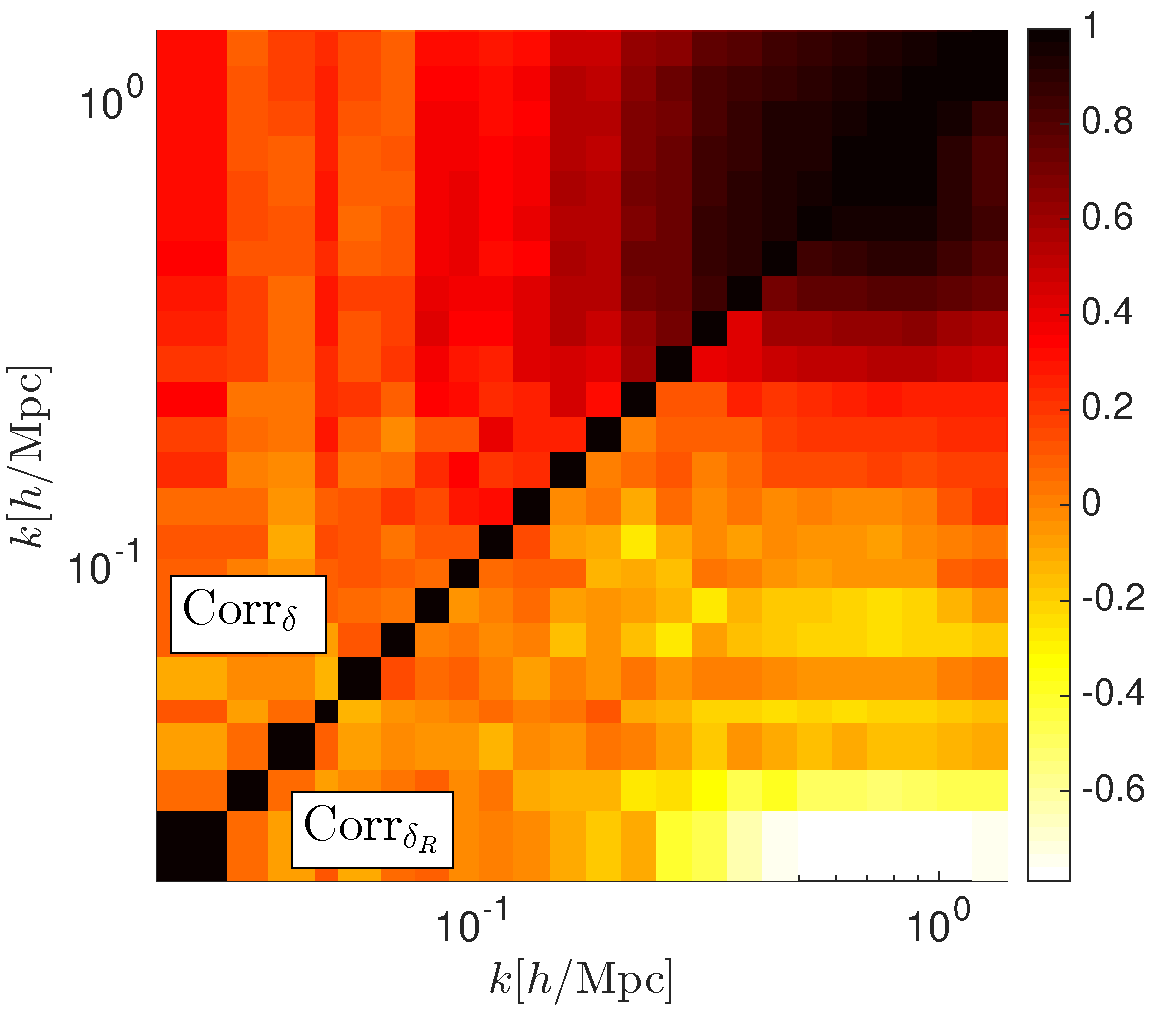
\includegraphics[width=0.48\textwidth]{corrmat_hot_2-crop.pdf}
%  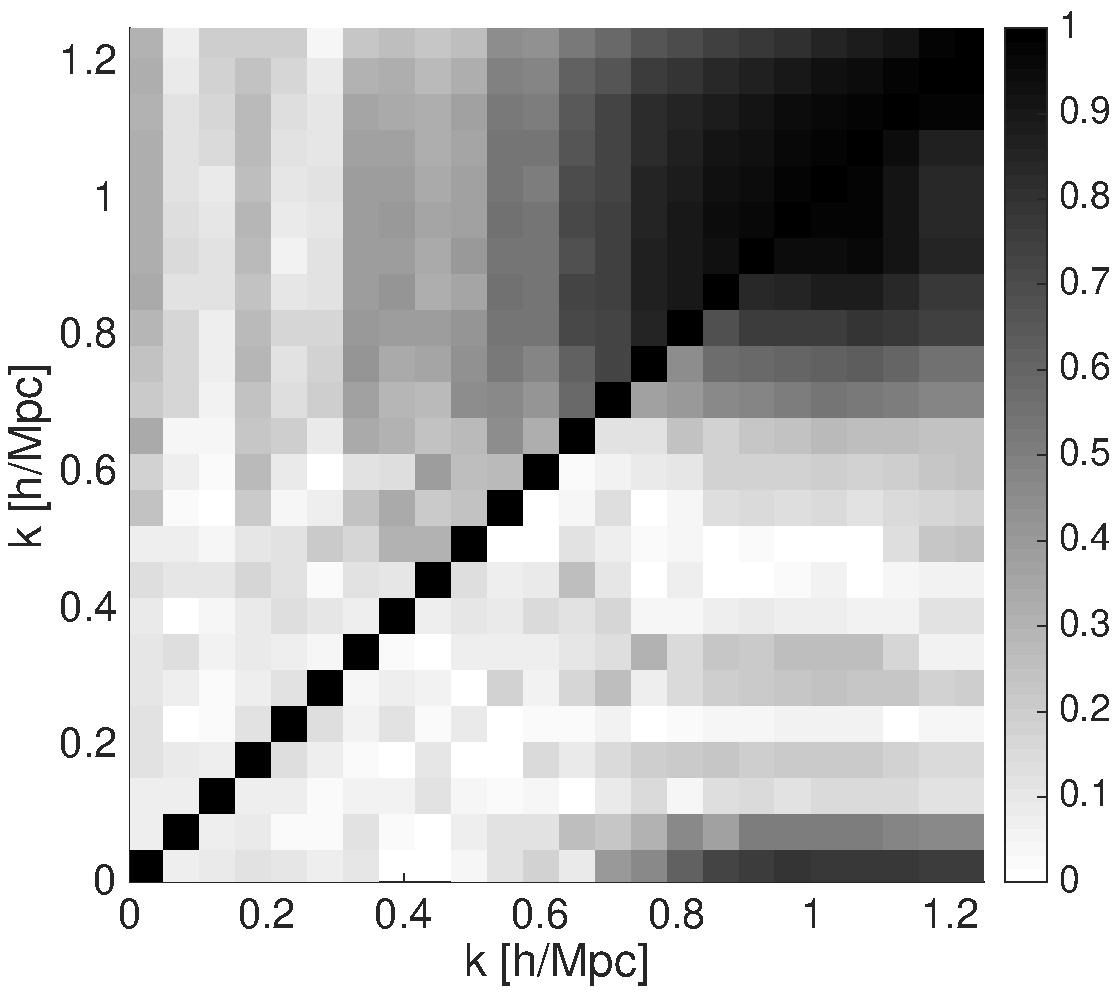
\includegraphics[width=0.48\textwidth]{corr_cut-crop.pdf}
  \caption{Correlation coefficient matrix as found from 136 nonlinear power spectra 
(the upper-left elements) and the reconstructed power spectra (the lower-right off-diagonal elements). 
Both the matrix are symmetric and have unity diagonal elements.}
    \label{fig:corrall}
\end{figure}

%  The signal-to-noise ratio, sometimes also called Fisher information, can be given by the inverse matrix of covariance. Since the signal-to-noise ratio was given in some work, we also present it for a better comparison. 
%\begin{align}
%\left( \frac{S}{N}\right)^2 (k_{n}) =\sum_{i,j=1}^n P_i \mathrm{Cov}^{-1}(i,j) P_j
%\end{align}

  Cumulative Fisher information is proportional to the volume. We plot the 
cumulative Fisher information per volume of the nonlinear, linear and reconstructed power specta in 
Fig.\ref{fig:fisherinfo}(a). The Fisher information of the nonlinear power spectra drops 
from the linear one at $k \simeq$ 0.05 $h/\mathrm{Mpc}$, and has a flat plateau in the translinear regime, 
$k\simeq$ 0.3 $h/\mathrm{Mpc}$, with 
a saturated value of $I \simeq 2.5 \times 10^{-5}/(\mathrm{Mpc}^3/h^3)$. It 
indicates that there is nearly no independent information of the power
spectrum in the translinear regime.
% At $k\sim0.8$, the information increase slightly aggain. 
But the information curve of 
the reconstructed power spectra keeps increasing roughly the same as 
the linear information until $k\simeq$ 0.3 $h/\mathrm{Mpc}$, and reaches its plateau at $k\simeq$ 0.8 $h/\mathrm{Mpc}$ with the 
value of $I \simeq  10^{-3}/(\mathrm{Mpc}^3/h^3)$, up by a factor of  40. 
It indicates that the MM reconstructed method can strongly recover the lost information 
within this scale. We compare the Fisher information given by the MM reconstruction method with 
the logarithmic density mapping method \cite{bib:Mark2009} as an example to illustrate their strength. 
We find that the MM reconstruction gives more than 10 times more information than logarithmic mapping. 
In some papers, the cross correlation $r^2$ terms are set to be unity in Eq.\ref{eq:fisherformulaused}, which 
apparantly increases the nonlinear information. We also plot those in Fig.\ref{fig:fisherinfo}(b) 
for better comparison. But we find that in this case, the MM reconstructed and logarithmic mapping information 
is higher than the linear one in the scale 
$k \simeq$ 0.2 - 0.5 $h/\mathrm{Mpc}$, which is not expected. 
\begin{figure*}
%\begin{subfigure}[b]{0.48\textwidth}
%\centering
  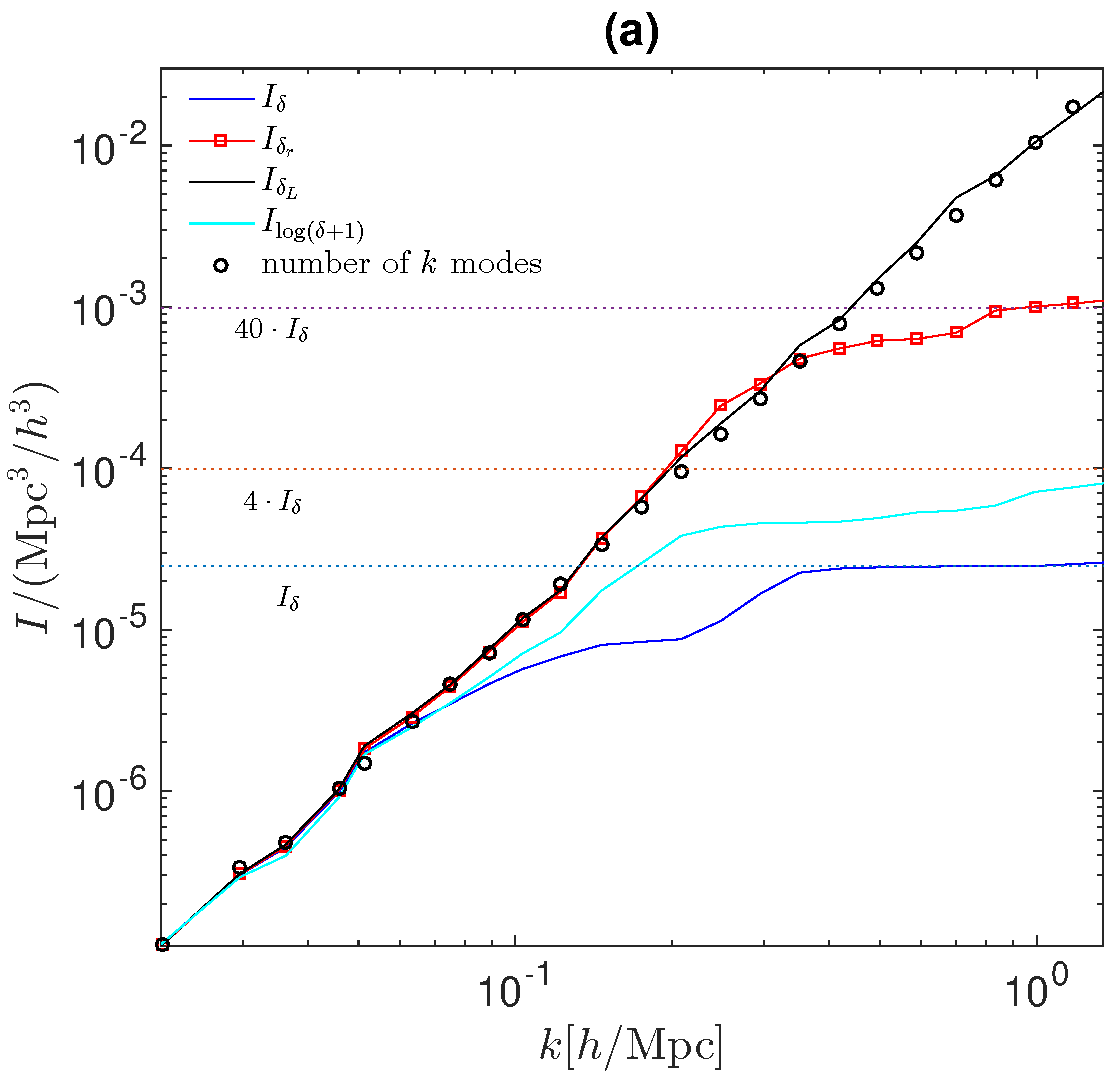
\includegraphics[width=0.5\textwidth]{fisher_r2_best_analysis-crop.pdf}
%\end{figure}
%\begin{subfigure}[b]{0.48\textwidth}
%\bebin{subfigure}
%\centering
  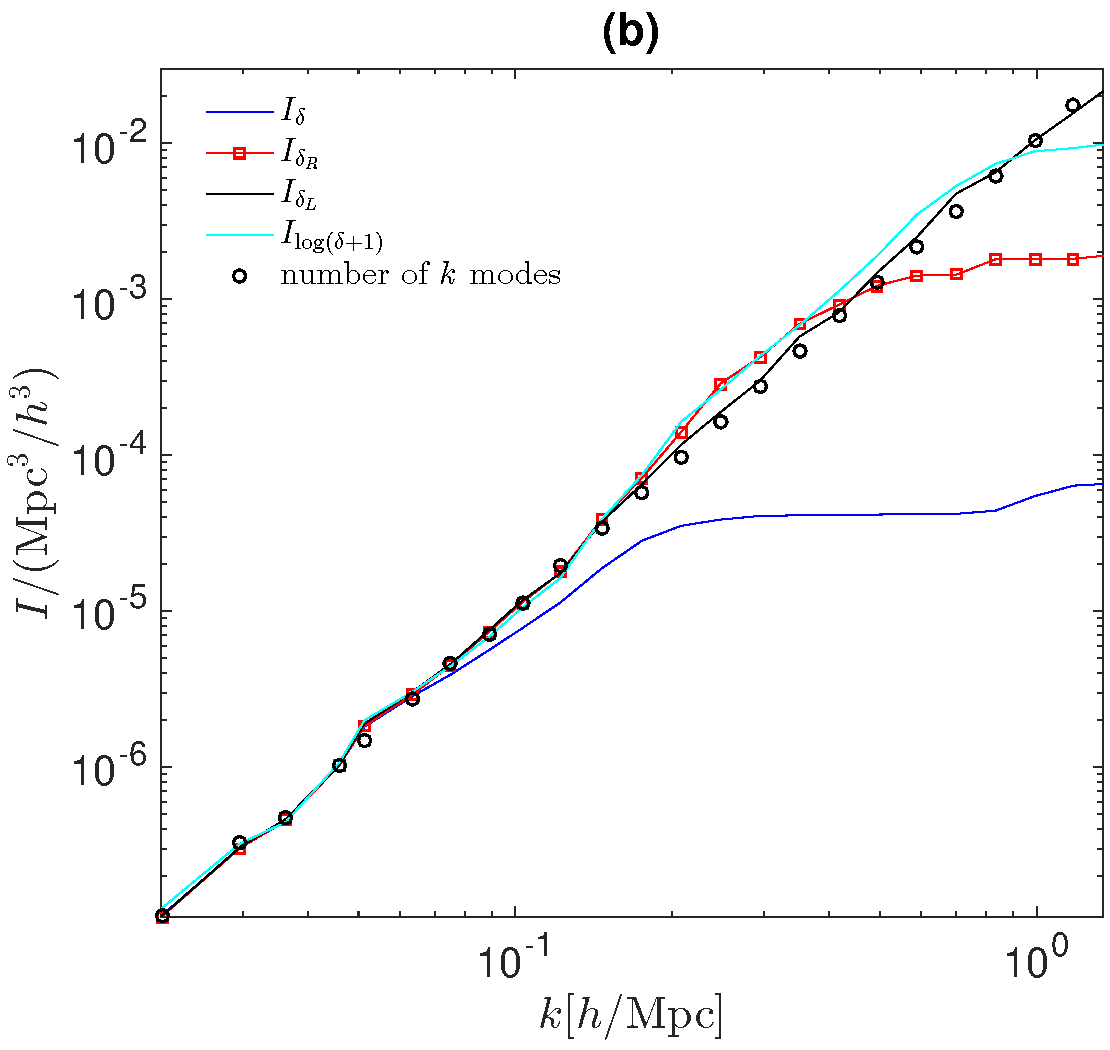
\includegraphics[width=0.46\textwidth]{fisher_best_analysis-crop.pdf}
%\end{subfigure}
%  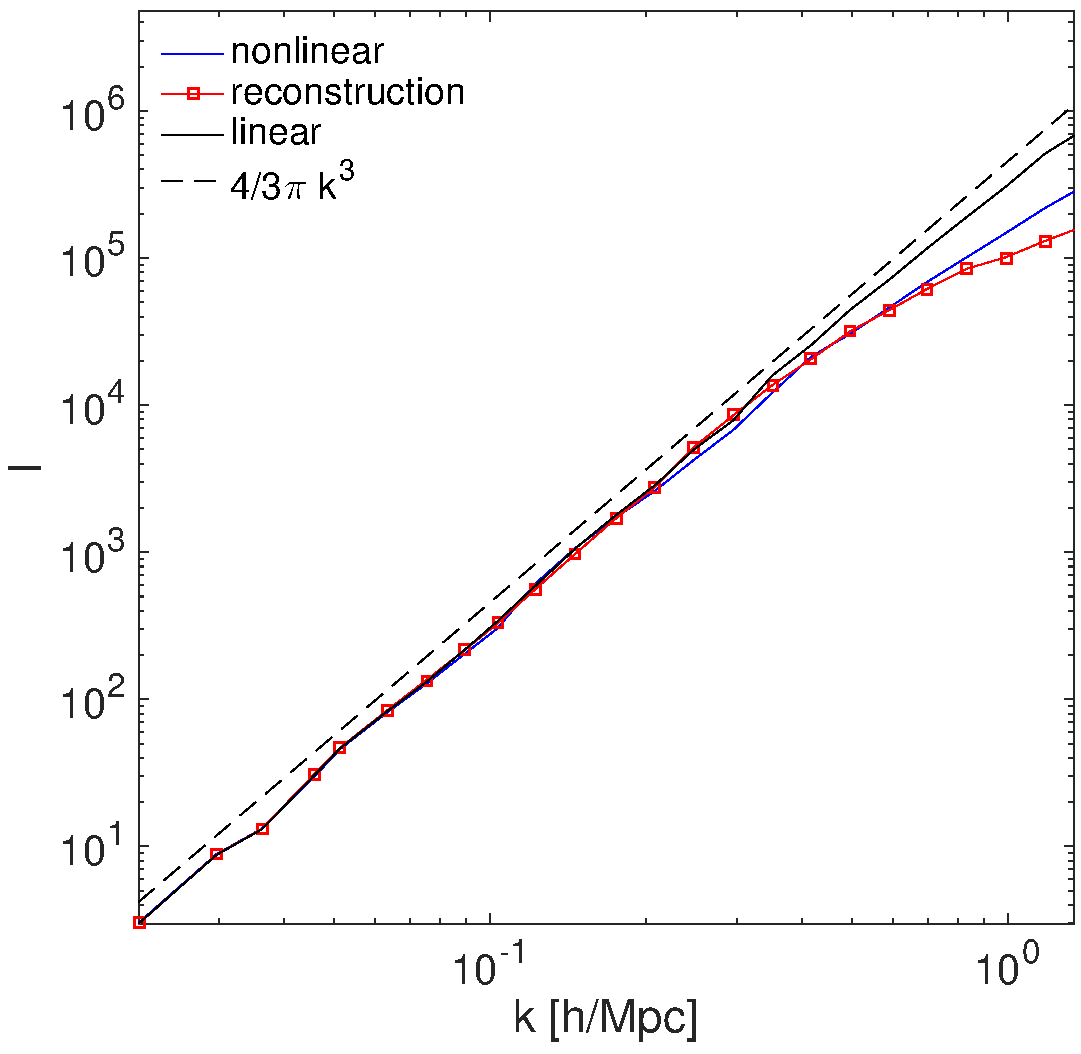
\includegraphics[width=0.48\textwidth]{fisher_tr-crop.pdf}
%  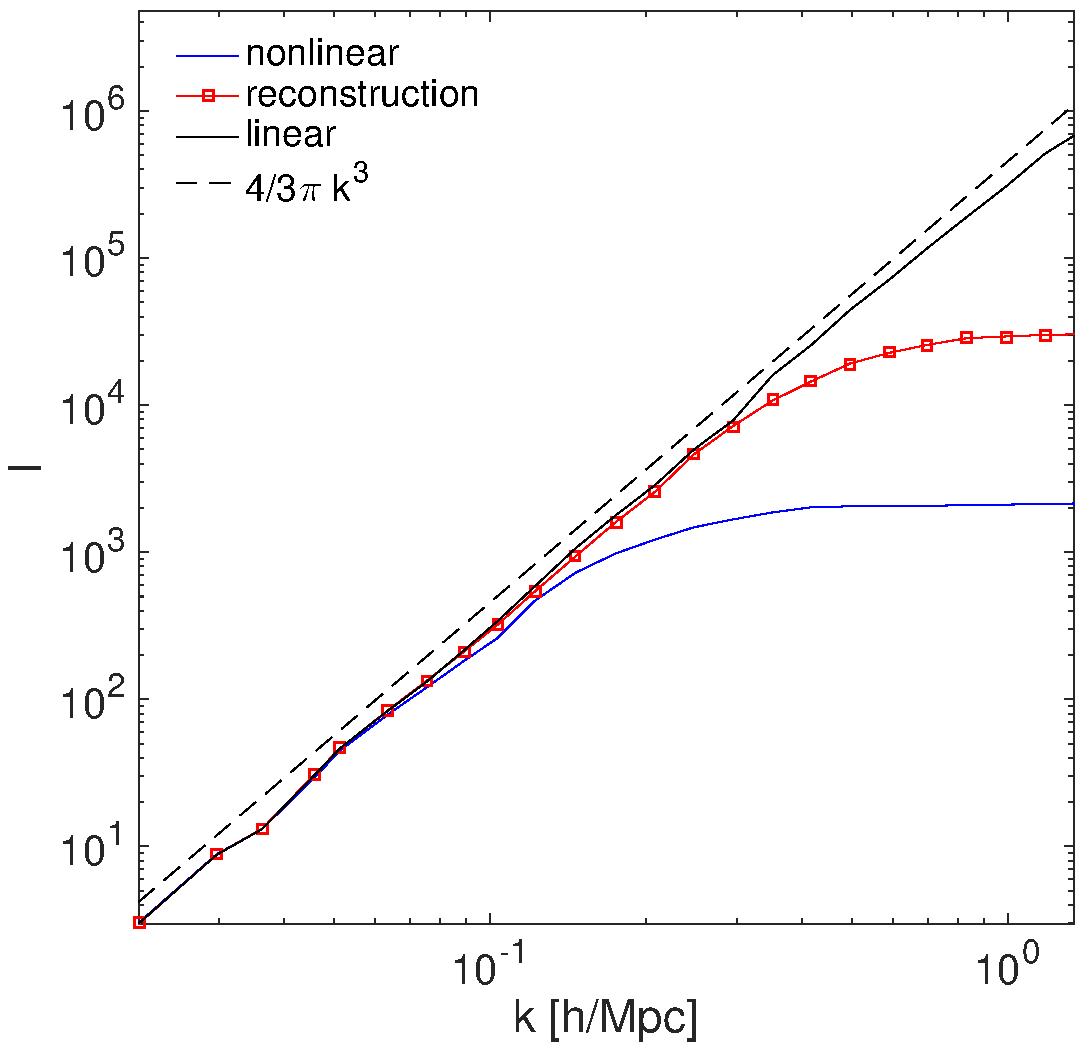
\includegraphics[width=0.48\textwidth]{fisher_trr2-crop.pdf}
\centering
   \caption{(a) Cumulative Fisher information per volume in the power spectra 
as a function of wavenumber. The blue line corresponds to the nonlinear density fields; 
the red line with squares corresponds to the the reconstructed density fields; 
the dark line corresponds to the linear density fields; the circles correspond to number 
of $k$ modes up to that wave bin. Dotted lines correspond to saturated value of 
nonlinear Fisher information, 4 times and 40 times of it, respectively. (b) Cumulative Fisher information 
per volume given by setting the cross correlation to be unity.}
  \label{fig:fisherinfo}

\end{figure*}
%\begin{figure*}
%[htbp]
% \centering
%  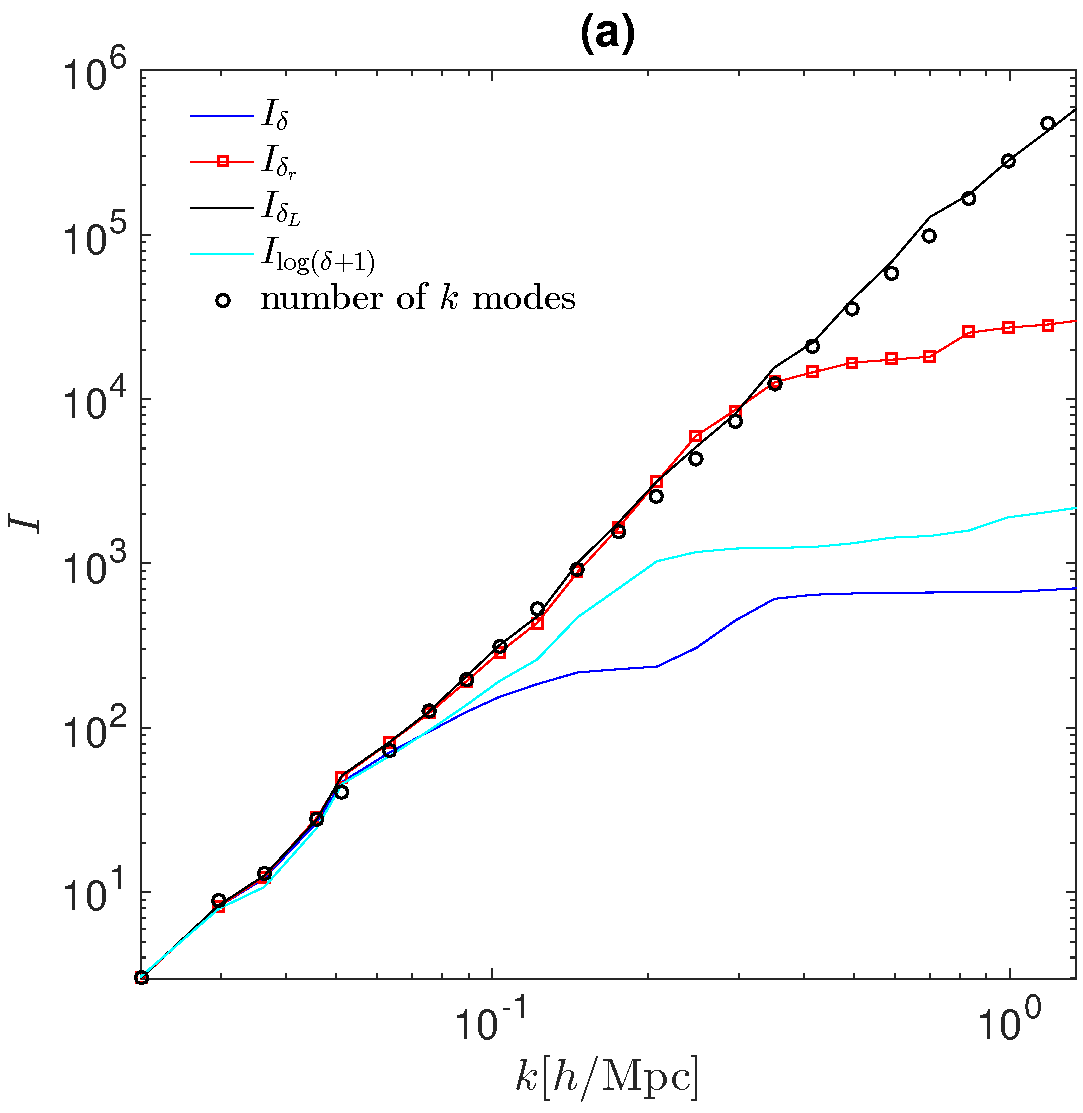
\includegraphics[width=0.48\textwidth]{fisher_addlog_r2-crop.pdf}
%  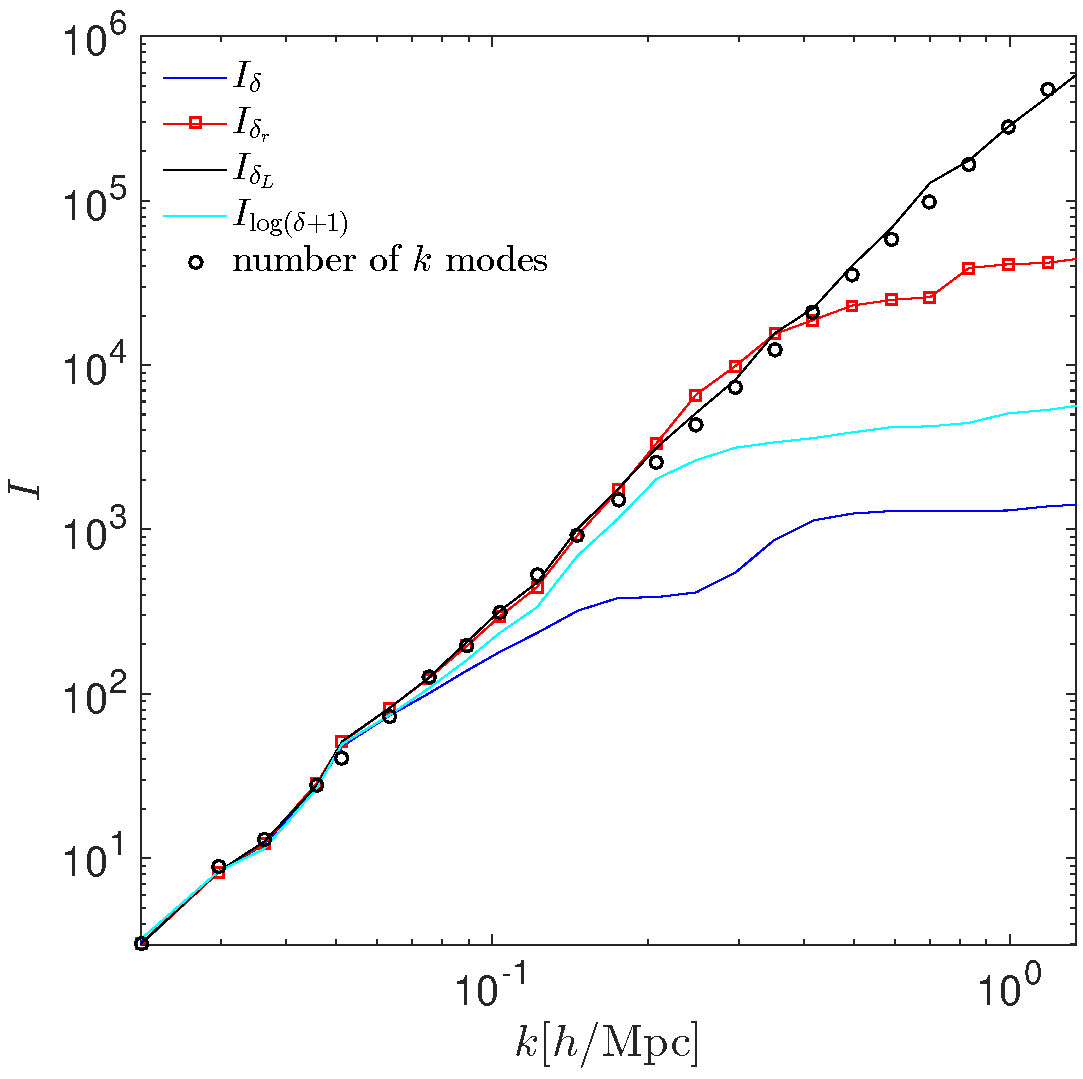
\includegraphics[width=0.48\textwidth]{fisher_addlog_r-crop.pdf}
%  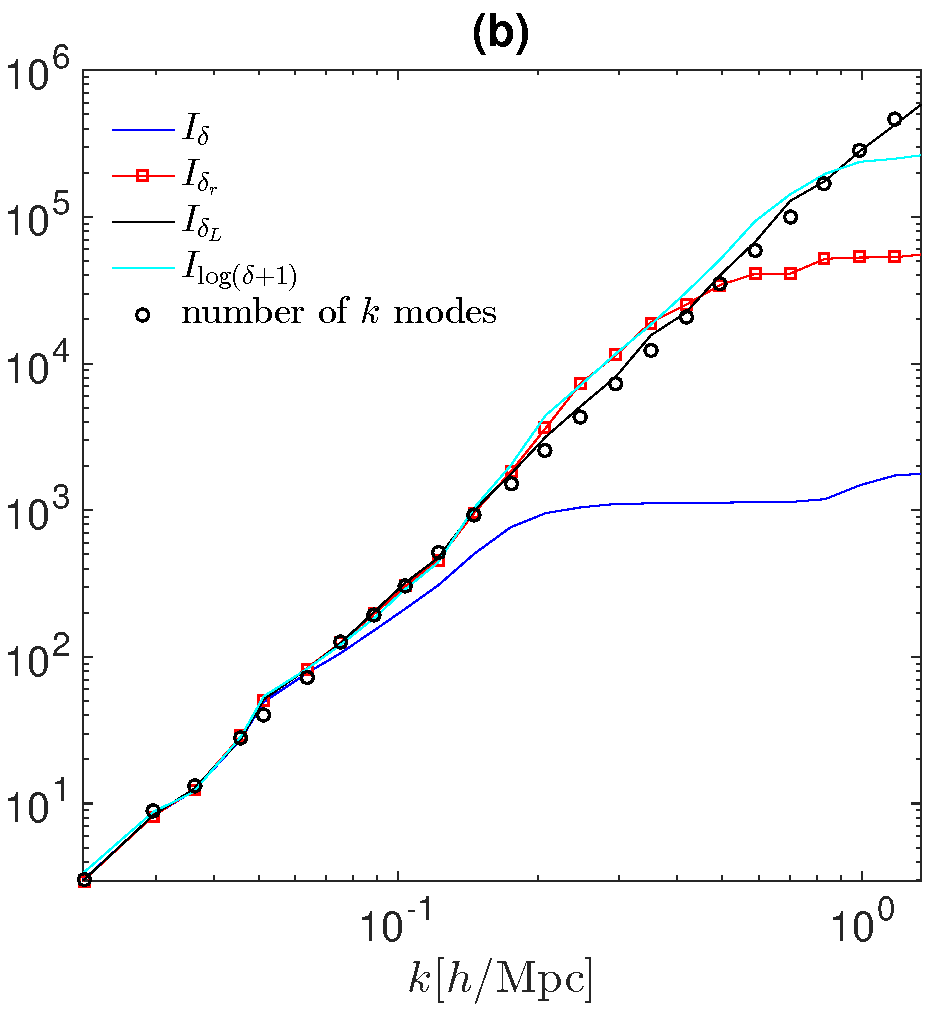
\includegraphics[width=0.48\textwidth]{fisher_addlog-crop.pdf}
%\caption{1:$r^2$; 2:$r$; 3:old version}
%  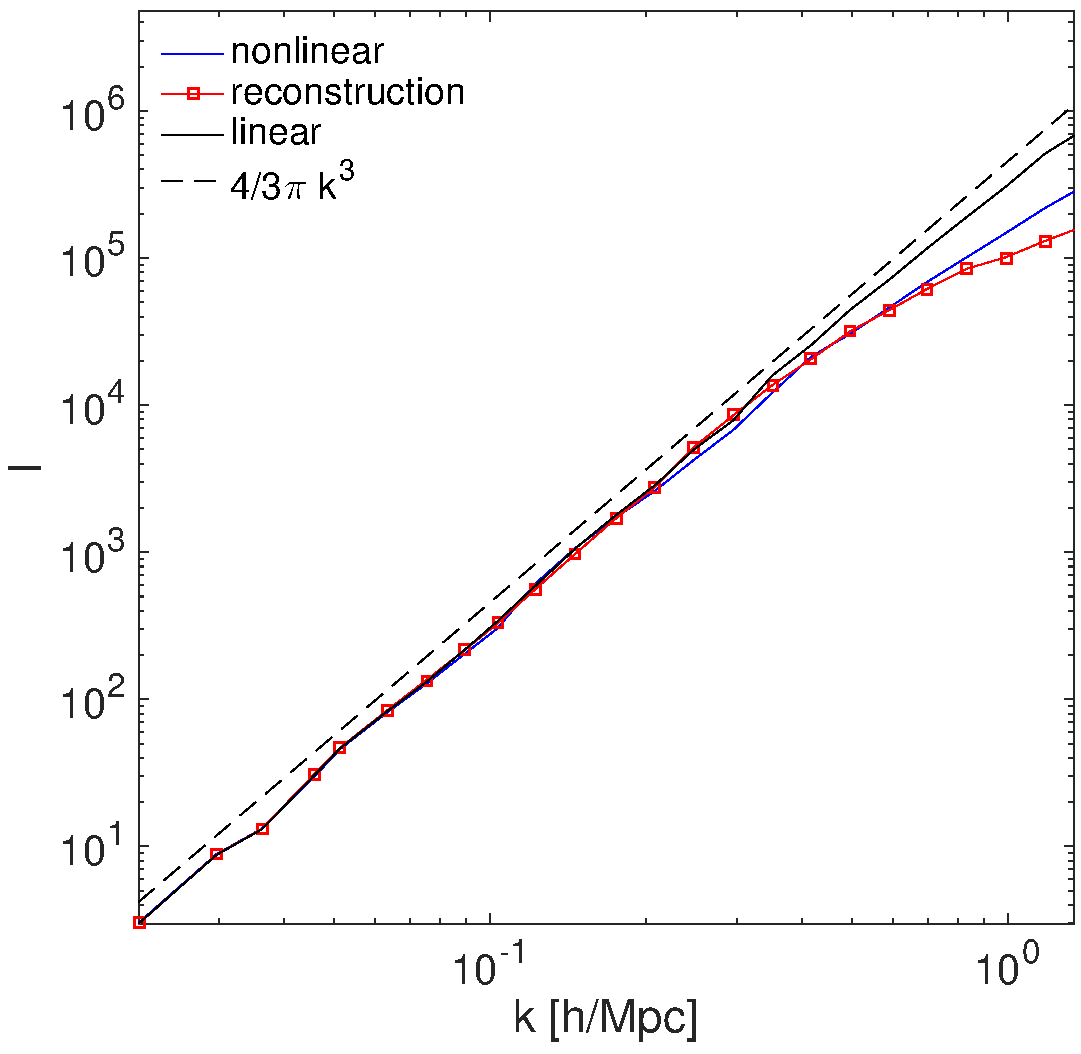
\includegraphics[width=0.48\textwidth]{fisher_tr-crop.pdf}
%  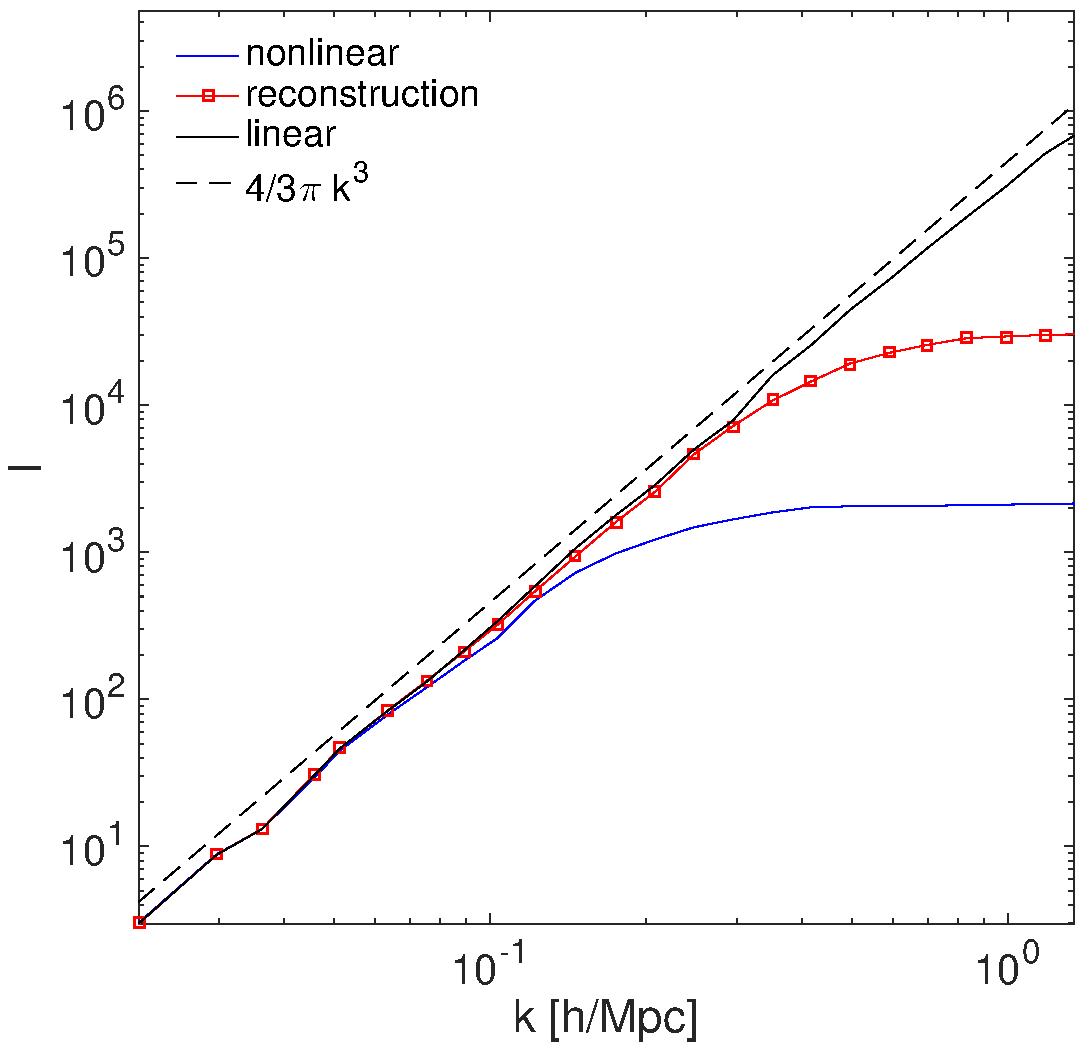
\includegraphics[width=0.48\textwidth]{fisher_trr2-crop.pdf}
%\end{figure*}
%\begin{figure*}
%\centering
%  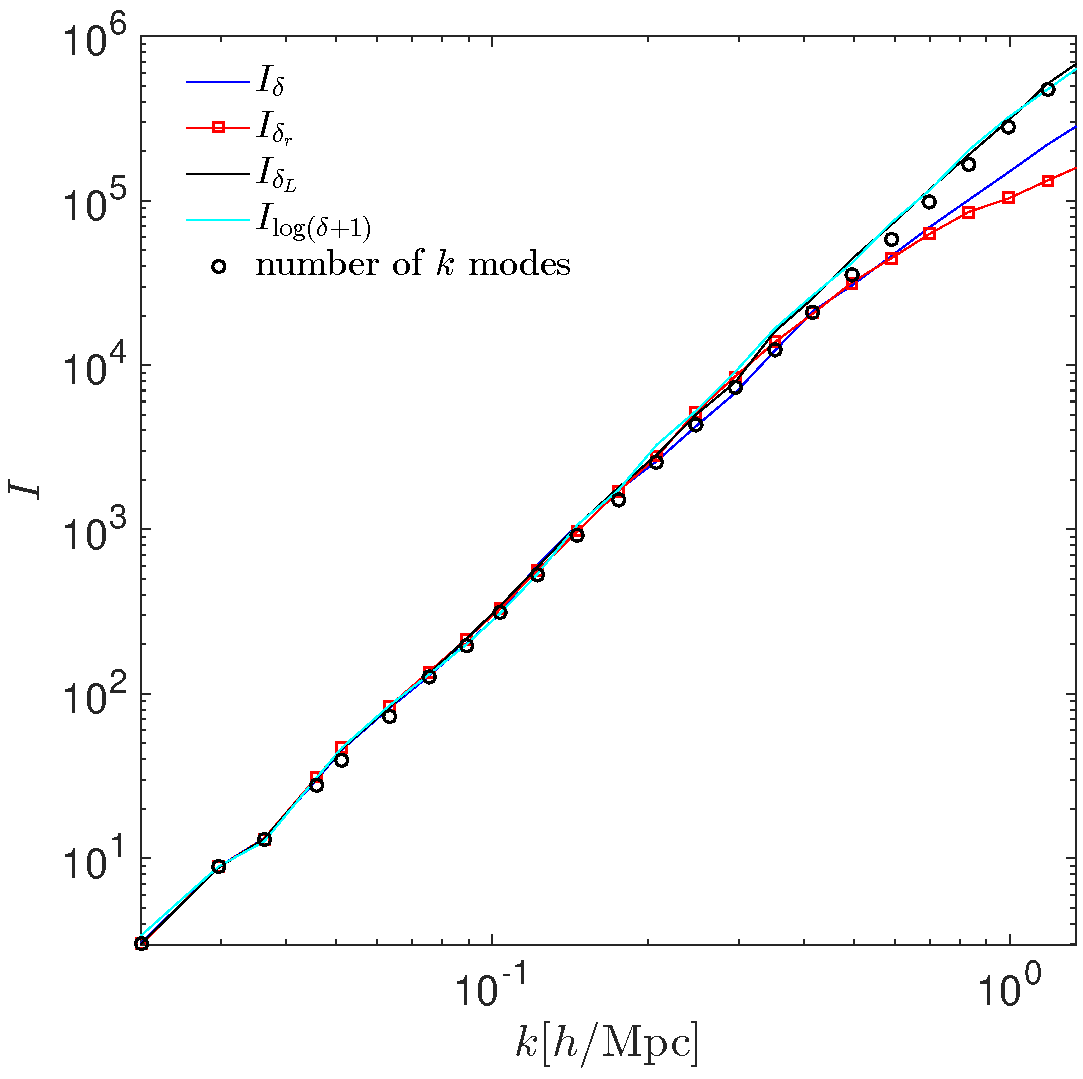
\includegraphics[width=0.48\textwidth]{fisher_addlog_diag-crop.pdf}
%  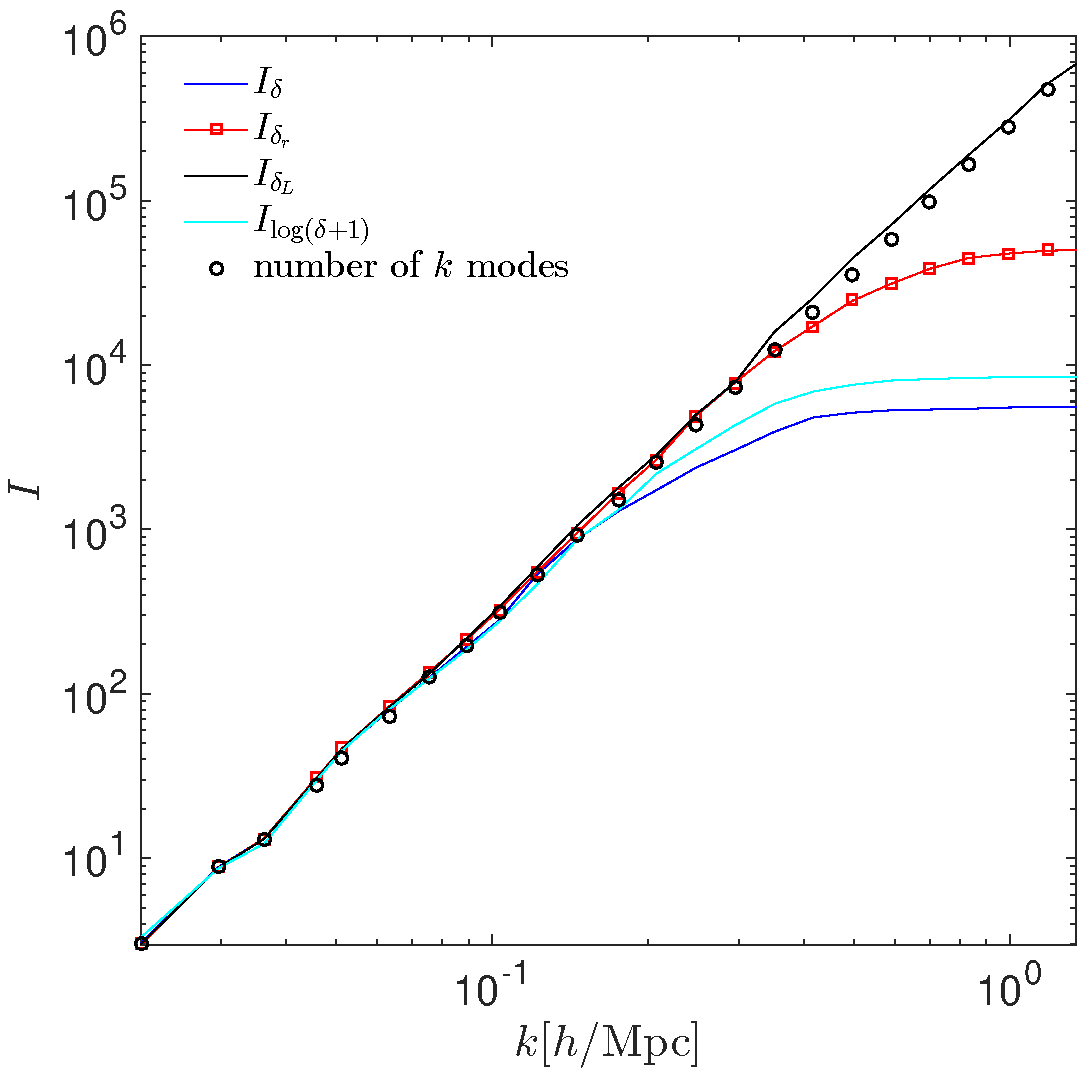
\includegraphics[width=0.48\textwidth]{fisher_addlog_diagr-crop.pdf}
%  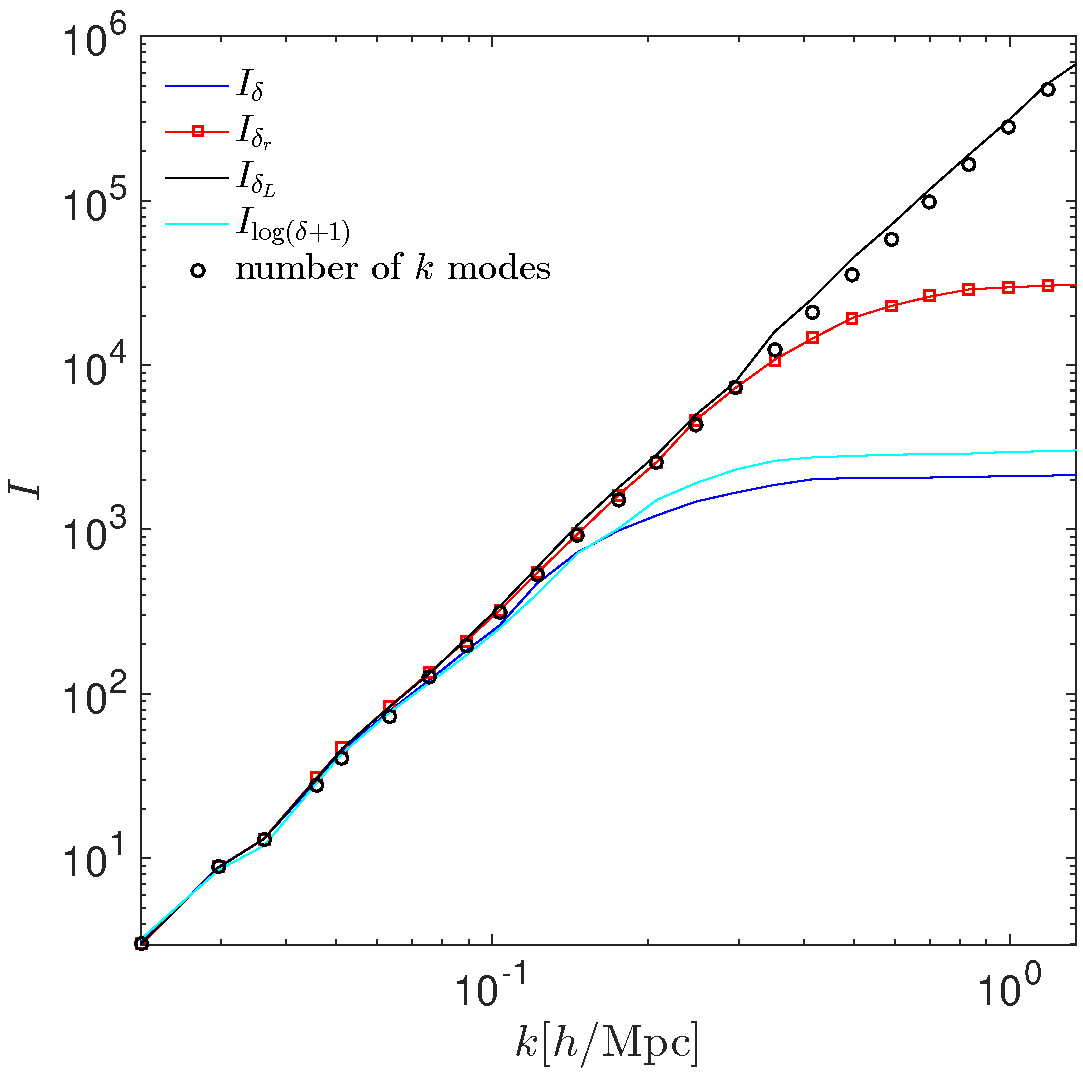
\includegraphics[width=0.48\textwidth]{fisher_addlog_diagr2-crop.pdf}
%\caption{1: diag; 2: diag*$r$, 3: diag*$r^2$}
%\end{figure*}

\end{section}
